\documentclass[12pt]{article}

% === Packages ===
\usepackage[utf8]{inputenc}
\usepackage[T1]{fontenc}
\usepackage{lmodern}
\usepackage[margin=1in]{geometry}
\usepackage{amsmath,amssymb}
\usepackage{graphicx}
\usepackage{booktabs}
\usepackage{tabularx}
\usepackage{xcolor}
\usepackage[round]{natbib}
\usepackage[colorlinks=true,linkcolor=blue!60!black,citecolor=blue!60!black,urlcolor=blue!60!black]{hyperref}
\usepackage{microtype}
\usepackage{setspace}
\usepackage{parskip}

% === Formatting ===
\onehalfspacing

% === Title ===
\title{The Four-Model Theory of Consciousness:\\A Simulation-Based Framework Unifying the Hard Problem, Binding, and Altered States}
\author{Matthias Gruber\\
\textit{Independent researcher}\\
ORCID: \href{https://orcid.org/0009-0005-9697-1665}{0009-0005-9697-1665}\\
\texttt{matthias@matthiasgruber.com}}
\date{}

% === Document ===
\begin{document}
\maketitle

\begin{abstract}\singlespacing
This paper presents the Four-Model Theory, in which consciousness is constituted by real-time self-simulation across four nested models arranged along two axes---scope (world vs.\ self) and mode (implicit vs.\ explicit). The implicit models (Implicit World Model, Implicit Self Model) are substrate-level, learned, and non-conscious. The explicit models (Explicit World Model, Explicit Self Model) are virtual, transient, and phenomenal---the simulation in which experience occurs. The central claim is that qualia are virtual: they exist within and are constitutive of the simulation, not properties of the physical substrate. This dissolves the Hard Problem by revealing a category error---the physical processing does not feel; the simulation does. Combined with a criticality requirement (the substrate must operate at the edge of chaos), the theory derives diverse phenomena from five principles: criticality, virtual qualia, a redirectable Explicit Self Model, variable implicit--explicit permeability, and virtual model forking. These unify psychedelic phenomenology, anesthetic mechanisms, dream states, split-brain phenomena, dissociative identity disorder, and animal consciousness. A systematic comparison shows the theory addresses all eight core requirements a complete theory of consciousness must meet. Nine novel testable predictions are offered, including that psychedelic ego dissolution content is controllable via sensory input and that psychedelics should alleviate anosognosia---predictions no competing theory generates. The criticality requirement, independently derived from Wolfram's computational framework in 2015, converges with empirical criticality literature consolidated in 2025--2026 \citep{HengenShew2025,AlgomShriki2026}.
\end{abstract}

\noindent\textbf{Keywords}: consciousness, hard problem, self-model, simulation, qualia, criticality, binding problem, altered states, psychedelics, substrate independence

%=============================================================================
\section{Introduction}
%=============================================================================

\subsection{The Pre-Paradigm State of Consciousness Science}

After three decades of intensive investigation, consciousness research finds itself at an impasse. The field possesses no dominant paradigm in the Kuhnian sense \citep{Kuhn1962}, no agreed-upon methodology for linking subjective experience to objective measurement, and no theory that commands broad assent. Multiple frameworks compete---Integrated Information Theory (IIT; \citealp{Tononi2004}; \citealp{Albantakis2023}), Global Neuronal Workspace (GNW; \citealp{Baars1988}; \citealp{Dehaene2011}), Higher-Order Theories (HOT; \citealp{Rosenthal2005}; \citealp{Lau2011}), Predictive Processing (PP; \citealp{Seth2021}), Attention Schema Theory (AST; \citealp{Graziano2013}), Recurrent Processing Theory (RPT; \citealp{Lamme2006})---yet none has established decisive superiority.

Recent developments have deepened the crisis. The COGITATE adversarial collaboration published equivocal results \citep{Melloni2023,COGITATE2025}: neither IIT nor GNW was fully confirmed. A letter signed by over 100 researchers declared IIT pseudoscientific \citep{NatNeuro2025IIT}, provoking fierce rebuttals \citep{Konstantinou2025}.

This paper argues that the impasse persists because no existing theory simultaneously addresses all fundamental requirements a complete theory must meet. Each theory excels on some requirements but remains silent on, or weak against, others.

\subsection{What Would Count as Progress?}

I propose that any theory claiming to provide a comprehensive account of consciousness must address eight core requirements, drawn from the philosophical and scientific literature. These requirements are not novel; each has been identified by previous authors as a central challenge. What is novel is the demand that a single theory address all eight simultaneously:

\begin{enumerate}
\item \textbf{The Hard Problem} \citep{Chalmers1995}---Why does physical processing give rise to subjective experience?
\item \textbf{The Explanatory Gap} \citep{Levine1983}---Why does the explanation of neural correlates feel incomplete?
\item \textbf{The Boundary Problem} \citep{Bayne2010,Tononi2004}---Where does the conscious system end?
\item \textbf{The Structure of Experience} \citep{Nagel1974}---How does physical processing produce richly structured experience?
\item \textbf{Unity and Binding} \citep{Treisman1980,Revonsuo1999}---How are distributed processes unified into coherent experience?
\item \textbf{Combination and Emergence} \citep{Chalmers2016}---How do non-conscious elements combine to produce consciousness?
\item \textbf{The Causal Role} \citep{Jackson1982}---Does consciousness do anything?
\item \textbf{The Meta-Problem} \citep{Chalmers2018}---Why do we think there is a hard problem?
\end{enumerate}

Section~2 develops each requirement in detail and surveys how existing theories fare against them. The remainder of the paper presents a theory---the Four-Model Theory---that, I argue, addresses all eight.

\subsection{Overview and Historical Context}

The Four-Model Theory was originally published in German as \textit{Die Emergenz des Bewusstseins} \citep{Gruber2015} and refined through structured adversarial challenge in 2026. It draws on Dennett's Multiple Drafts Model \citep{Dennett1991}, Metzinger's Self-Model Theory \citep{Metzinger2003,Metzinger2009}, and neural network architecture, proposing that consciousness consists of a real-time self-simulation running on an implicit knowledge base. Qualia are virtual: they exist within the simulation but not at the substrate level. This two-level ontology dissolves the Hard Problem by showing it rests on a category error. Combined with a criticality requirement derived from Wolfram's computational framework \citep{Wolfram2002}, the theory generates nine testable predictions and unifies phenomena across psychopharmacology, clinical neurology, sleep science, and comparative cognition.

%=============================================================================
\section{Eight Requirements for a Theory of Consciousness}
%=============================================================================

Any theory claiming to provide a comprehensive account must address eight core requirements drawn from the philosophical and scientific literature. A detailed theory-by-theory comparison follows in Section~7; the purpose here is to establish the evaluative framework.

\subsection{The Hard Problem}

\citet{Chalmers1995,Chalmers1996} asked why physical processing is accompanied by subjective experience. We can explain all the \textit{functions} of consciousness without explaining why there is ``something it is like'' \citep{Nagel1974} to undergo these processes. Most neuroscientific theories (GNW, RPT, PP) remain silent on this. IIT addresses it by identifying consciousness with integrated information ($\Phi$), but this requires panpsychist commitments \citep{Aaronson2014,Doerig2019}. Illusionism \citep{Dennett1991,Frankish2016} dissolves the problem by denying qualia exist---a position that remains controversial.

\subsection{The Explanatory Gap}

\citet{Levine1983} identified a gap between third-person neural descriptions and first-person experience. \citet{Block1995,Block2007} refined this as the distinction between access and phenomenal consciousness. The Explanatory Gap has a distinct character from the Hard Problem: it concerns the \textit{form} of explanation rather than the \textit{existence} of the phenomenon.

\subsection{The Boundary Problem}

Where does the conscious system begin and end? Within the brain, only some processing is conscious at any given moment; between organisms, it is unclear where to draw the line. IIT's exclusion postulate (the system with maximum $\Phi$ defines the boundary) provides the strongest treatment but is computationally intractable. GNW defines access via global broadcasting, but the boundary between broadcast and non-broadcast content is not always sharp. PP uses Markov blankets \citep{Friston2010} but may be too liberal \citep{Bruineberg2022}.

\subsection{The Structure of Experience}

Conscious experience has rich spatial, temporal, modal, and qualitative structure---colors, shapes, pitches, emotional valence, phenomenal character. Any complete theory must explain how physical processing generates this structured phenomenology. IIT's qualia space provides a mathematical treatment (arguably IIT's greatest strength); PP's generative models are inherently structured. GNW and HOT are weaker here, explaining \textit{when} content becomes conscious but less about \textit{why} it has specific structure.

\subsection{Unity and Binding}

The Binding Problem \citep{Treisman1996,Revonsuo1999} asks how distributed neural processes---in different brain regions, at different timescales, in different modalities---are unified into coherent experience. Proposed solutions range from temporal synchrony \citep{Fries2005,Fries2015} to integrated information \citep{Tononi2004} to global broadcasting \citep{Baars1988}. None is universally accepted.

\subsection{Combination and Emergence}

How do non-conscious elements combine to produce consciousness? Panpsychist theories face the Combination Problem \citep{Chalmers2016,Coleman2014}: how do micro-experiences combine into macro-experience? Physicalist theories face the objection that they invoke either strong emergence (mysterious) or functional reduction (inadequate).

\subsection{The Causal Role of Consciousness}

Does consciousness \textit{do} anything, or is it epiphenomenal? Epiphenomenalism \citep{Huxley1874,Jackson1982} is widely dismissed, yet mechanistic theories struggle to specify what role \textit{experience} plays beyond mechanism. PP's active inference provides the strongest existing case for a functional role.

\subsection{The Meta-Problem}

Why do we \textit{think} there is a Hard Problem \citep{Chalmers2018}? Even if the Hard Problem is illusory, the fact that most humans report a strong intuition that consciousness is mysterious requires explanation. AST provides the strongest account: the self-model of attention necessarily omits mechanistic details, producing the intuition of mystery \citep{Graziano2013}. However, AST explains why we \textit{think} there is a mystery without accounting for the mystery itself.

%=============================================================================
\section{The Four-Model Theory}
%=============================================================================

\subsection{Core Definition}

Consciousness is the ability of an entity---biological or artificial---to create a model of itself, to relate that model to itself, and to interact with it. Consciousness is not a property the brain possesses but a process the brain performs: it runs a real-time self-simulation.

This definition is functional and substrate-independent. It does not require a specific physical implementation, biological composition, or computational architecture. What it requires is a system capable of constructing and maintaining a self-referential simulation in real time.

\subsection{The Four Models}

The theory identifies four nested models distinguished by two orthogonal dimensions: \textbf{scope} (everything vs.\ self only) and \textbf{mode} (implicit/learned vs.\ explicit/simulated). This is a conceptual taxonomy, not a claim about spatial organization in the brain---the models are functionally distinct processes, not anatomically localized regions.

\begin{table}[htbp]
\centering
\caption{The Four-Model Architecture}
\label{tab:four-models}
\begin{tabularx}{\textwidth}{lXX}
\toprule
& \textbf{Everything (world)} & \textbf{Self only} \\
\midrule
\textbf{Implicit} (learned, substrate-level) & Implicit World Model (IWM) & Implicit Self Model (ISM) \\
\textbf{Explicit} (simulated, phenomenal) & Explicit World Model (EWM) & Explicit Self Model (ESM) \\
\bottomrule
\end{tabularx}
\end{table}

\begin{figure}[htbp]
\centering
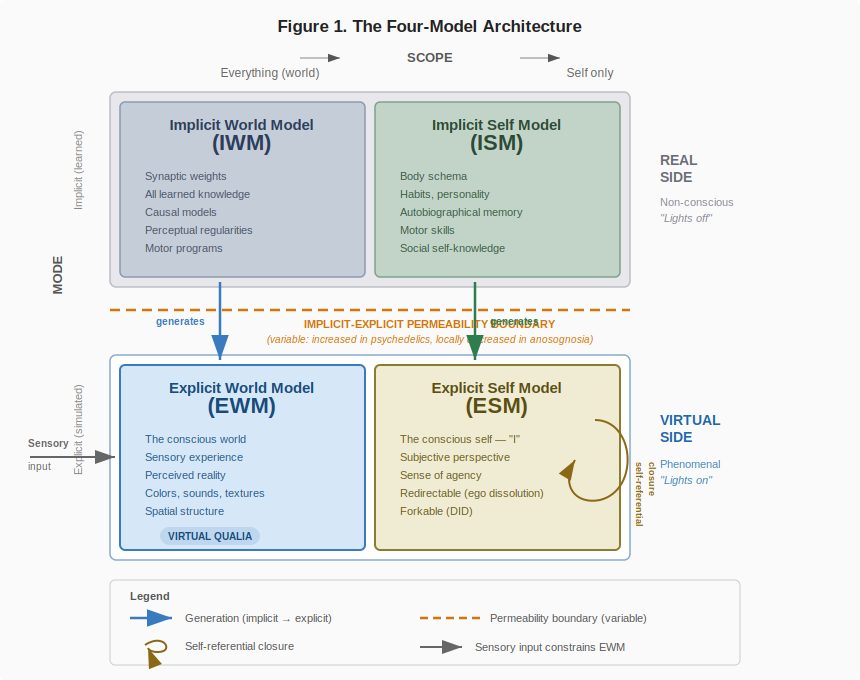
\includegraphics[width=0.85\textwidth]{figure1-four-model-architecture.png}
\caption{The four-model architecture. The two orthogonal axes---scope (world vs.\ self) and mode (implicit vs.\ explicit)---define four functionally distinct models. Implicit models (bottom) are substrate-level, learned, and non-conscious. Explicit models (top) are virtual, transient, and phenomenal.}
\label{fig:four-models}
\end{figure}

\textbf{The Implicit World Model (IWM)} encompasses the substrate's total accumulated knowledge about the world, stored in synaptic weights (or their functional equivalent in non-biological substrates). It includes everything the system has ever learned: perceptual regularities, causal models, spatial relationships, semantic knowledge, motor programs for interacting with the world. The IWM is never directly conscious. It operates ``in the dark''---providing the knowledge base from which the conscious simulation is generated, but never itself appearing in experience.

\textbf{The Implicit Self Model (ISM)} is the substrate's accumulated self-knowledge: body schema, proprioceptive calibration, motor skills, habits, personality traits, autobiographical memory structures, and social self-knowledge. Like the IWM, the ISM is never directly conscious. There is no unified homunculus---no inner observer reading the ISM. The ISM is a structural feature of the substrate, not an experiential one.

\textbf{The Explicit World Model (EWM)} is the conscious world---the real-time simulation of reality that constitutes perceptual experience. When you see a room, hear a voice, feel the texture of a surface, you are experiencing the EWM. It is generated from the IWM (which provides the world-knowledge) and current sensory input (which constrains and updates the simulation), but it is not identical to either. The EWM is a virtual construct---a transient pattern of activity, not a permanent structure.

\textbf{The Explicit Self Model (ESM)} is the conscious self---the real-time simulation of ``I'' that constitutes self-experience. It is the sense of being a subject, having a perspective, occupying a body, possessing a history, and being the author of one's actions. The ESM is generated from the ISM (which provides the self-knowledge) and current interoceptive and proprioceptive input, but like the EWM, it is virtual: a transient process, not a permanent entity.

\subsection{The Real/Virtual Split}

The four models divide into two fundamental categories:

\textbf{The real side} (IWM + ISM): These are physical, structural, learned, and non-conscious. They are stored in the substrate's architecture---in biological brains, primarily in synaptic weights, dendritic morphology, and connectivity patterns. They accumulate over the organism's lifetime through learning. They have no phenomenal character. ``Lights off.''

\textbf{The virtual side} (EWM + ESM): These are simulated, transient, generated, and phenomenal. They are patterns of activity---in biological brains, transient electrochemical dynamics. They are constructed in real time from the implicit models and current sensory input. They \textit{are} experience. ``Lights on.''

This division is the foundation of the theory's treatment of the Hard Problem (Section~3.4) and structures its account of every phenomenon it addresses.

\begin{figure}[htbp]
\centering
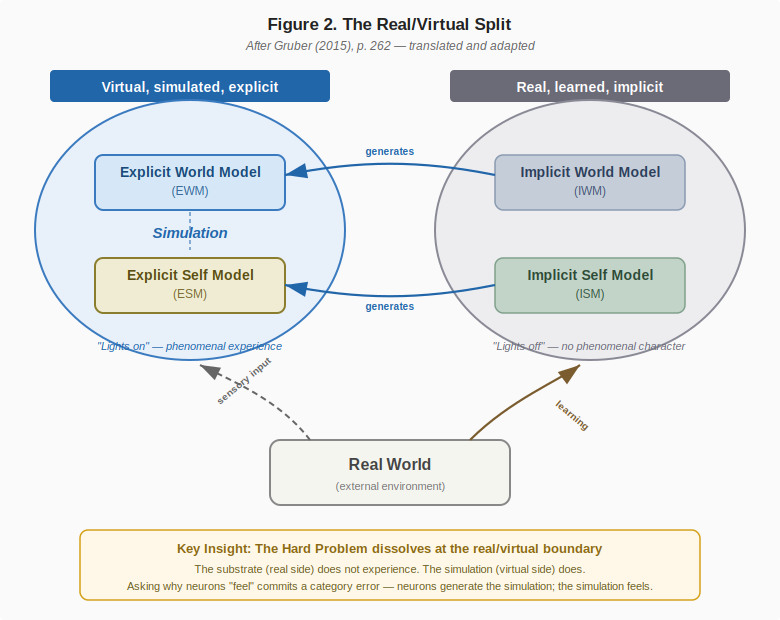
\includegraphics[width=0.85\textwidth]{figure2-real-virtual-split.png}
\caption{The ontological split between the real substrate (physical, structural, non-conscious---``lights off'') and the virtual phenomenal world (simulated, transient, experiential---``lights on''). Qualia exist only on the virtual side.}
\label{fig:real-virtual}
\end{figure}

The virtual models possess \textbf{software-like properties} that follow from their nature as simulations rather than structures:

\begin{itemize}
\item \textbf{They can be forked}: A single substrate can run multiple configurations of the ESM (see Section~6.2 on dissociative identity disorder).
\item \textbf{They can be cloned}: Physical separation of the substrate produces degraded but complete copies of the virtual models (see Section~6.4 on split-brain).
\item \textbf{They can be redirected}: The ESM requires input; disrupt normal self-referential input and it latches onto whatever input dominates (see Section~6.1 on psychedelics).
\item \textbf{They can be reconfigured}: Therapeutic interventions (CBT, exposure therapy) work by modifying the virtual models through substrate-level rewiring (see Section~6.6).
\end{itemize}

\subsection{Virtual Qualia: Dissolving the Hard Problem}

The central claim of the Four-Model Theory is that \textbf{qualia are virtual}. They are the way the simulated self (ESM) perceives its own states and the simulated world (EWM). Qualia exist within and are constitutive of the simulation; they do not exist at the substrate level.

This dissolves the Hard Problem by revealing a category error in its formulation:

\textbf{The standard formulation}: ``Why does physical processing (neuronal firing, synaptic transmission) feel like something?''

\textbf{The dissolution}: The physical processing \textit{does not} feel like anything. The IWM and ISM---the substrate-level implicit models---operate without any phenomenal character whatsoever. There is nothing it is like to be a synaptic weight. The simulation, however, \textit{does} feel---and within the simulation, qualia are simply what self-perception produces. Asking why neuronal firing feels like something is analogous to asking why transistor switching feels like running a video game. The transistors do not run the game at the level of individual switching; the virtual machine does. The neurons do not experience redness at the level of individual firing; the simulation does, and within the simulation, ``redness'' is simply the ESM's mode of registering a particular class of EWM content.

\textbf{Why self-simulation specifically?} A critic might object that this merely relocates the Hard Problem: why does \textit{this} virtual process have experience when a weather simulation does not? The answer lies in \textbf{self-referential closure}. A weather simulation models weather; it does not model \textit{itself modeling weather}. The four-model architecture creates a closed loop: the ESM models the system's own modeling process. In this loop, the distinction between model and modeled collapses---the simulation \textit{is} the thing being simulated. Qualia are not an \textit{addition} to self-modeling; they are self-modeling as encountered from the inside. A non-self-referential simulation has an outside from which it can be described without remainder; a self-referential simulation at criticality has no such outside. The simulation \textit{is} its own observer, and observation-from-inside is what we call experience.

This is not a proof that self-referential simulation must be conscious---it is an argument that self-referential simulation is the \textit{kind} of process for which the Hard Problem's assumptions break down. Self-referential closure is the condition under which the gap between process and feeling does not exist.

This is \textbf{not} illusionism \citep{Dennett1991,Frankish2016}. Illusionism denies that qualia exist. The Four-Model Theory holds that qualia are \textit{real within the simulation}---experience has genuine phenomenal character, but this character is a property of the virtual process, not of the physical substrate. This constitutes a \textbf{two-level ontology}: the substrate level has no experience, the simulation level has genuine experience. Both levels are physical, but they have different ontological properties. The Hard Problem's category error consists in seeking phenomenal properties at the substrate level where they do not exist.

The Explanatory Gap closes simultaneously. The gap between ``neurons fire in pattern X'' and ``I experience red'' reflects the level distinction: the firing pattern generates the simulation in which redness is experienced, but is not itself red, just as a CPU's electrical states are not ``a spreadsheet'' even though they generate one.

\subsection{Graduated Levels of Consciousness}

Consciousness is not binary but graduated, based on the depth of recursive self-modeling:

\textbf{Basic consciousness}: Minimal EWM and rudimentary ESM---phenomenal experience exists but self-awareness is thin. This is the entry level.

\textbf{Simply extended consciousness}: First-order self-observation. The system models itself---the ESM includes a model of the system's own states. The organism not only experiences but is aware that it experiences.

\textbf{Doubly extended consciousness}: Second-order self-observation. The system models itself modeling itself, enabling metacognition and the sense of being an observer of one's own mental processes.

\textbf{Triply extended consciousness}: Third-order self-observation. The system models itself modeling itself modeling itself. This supports philosophical reflection and the very intuition that consciousness is mysterious (the Meta-Problem). Only a system at this level can formulate the question ``What is consciousness?''

These levels are points on a continuum, not discrete stages. Different organisms occupy different positions, and individual organisms fluctuate between levels depending on state (waking, dreaming, meditative, intoxicated).

\subsection{The Implicit--Explicit Boundary}

A key mechanism is the \textbf{variable permeability of the boundary between implicit and explicit models}. Information becomes conscious when transferred from the implicit to the explicit side. In normal waking states, this boundary is selectively permeable: you are conscious of what the current simulation requires, not everything the implicit models contain.

Variation in permeability explains diverse phenomena (Section~6): psychedelic states involve global permeability increase (intermediate processing stages become accessible); anosognosia involves local permeability decrease (the ISM contains deficit information but transfer to the EWM is blocked); pre-sleep states involve gradually increasing permeability (producing the same visual progression as psychedelics); and meditation involves trained modulation of permeability.

\subsection{The Criticality Requirement}

The Four-Model Theory imposes a \textbf{physical prerequisite} for consciousness: the substrate must operate at or near the edge of chaos---Wolfram's Class~4 computational regime \citep{Wolfram2002}.

Wolfram classified cellular automata (and by extension computational systems generally) into four classes:
\begin{itemize}
\item \textbf{Class 1}: Converges to a fixed state. Too simple for consciousness.
\item \textbf{Class 2}: Periodic/repetitive. Too simple for consciousness.
\item \textbf{Class 3}: Chaotic/random. Too disordered for coherent consciousness.
\item \textbf{Class 4}: Complex/edge of chaos. Capable of universal computation. The regime in which consciousness can emerge.
\end{itemize}

This classification was applied to the question of consciousness in \citet{Gruber2015}, where it was argued that consciousness requires Class~4 dynamics---complex enough to sustain a self-simulation, ordered enough for that simulation to be coherent. This requirement was derived \textit{theoretically}, from the computational properties needed for real-time self-modeling, not from empirical neuroscience.

Independently, empirical neuroscience has converged on the same conclusion through a different path. \citet{Beggs2003} demonstrated neuronal avalanches consistent with self-organized criticality in cortical tissue. \citet{CarhartHarris2014} proposed the Entropic Brain Hypothesis, linking consciousness level to neural entropy. \citet{Tagliazucchi2012,Tagliazucchi2016} showed criticality signatures in waking fMRI and under LSD. \citet{Priesemann2013,Priesemann2014} characterized brain dynamics as slightly subcritical in normal waking states. This line of research was formally consolidated in the Consciousness and Criticality (ConCrit) framework \citep{AlgomShriki2026}, which synthesized evidence from 140 datasets across multiple paradigms to establish that consciousness tracks criticality across pharmacological, pathological, and physiological state changes.

\begin{table}[htbp]
\centering
\caption{Independent Convergence on Criticality}
\label{tab:criticality-convergence}
\begin{tabularx}{\textwidth}{lXl}
\toprule
\textbf{Year} & \textbf{Development} & \textbf{Path} \\
\midrule
2002 & Wolfram publishes \textit{A New Kind of Science} & Computational theory \\
2003 & Beggs \& Plenz---neuronal avalanches & Empirical neuroscience \\
2014 & Carhart-Harris---Entropic Brain Hypothesis & Empirical neuroscience \\
\textbf{2015} & \textbf{Gruber---Class~4 / edge of chaos requirement} & \textbf{Theoretical (via Wolfram)} \\
2016 & Tagliazucchi et al.---LSD and criticality & Empirical neuroscience \\
2022 & ``Self-organized criticality as a framework'' (review) & Empirical neuroscience \\
2025 & Hengen \& Shew---meta-analysis of 140 datasets & Empirical neuroscience \\
\textbf{2025--26} & \textbf{ConCrit framework (Algom \& Shriki)} & \textbf{Theoretical/empirical synthesis} \\
\bottomrule
\end{tabular}
\end{table}

\begin{figure}[htbp]
\centering
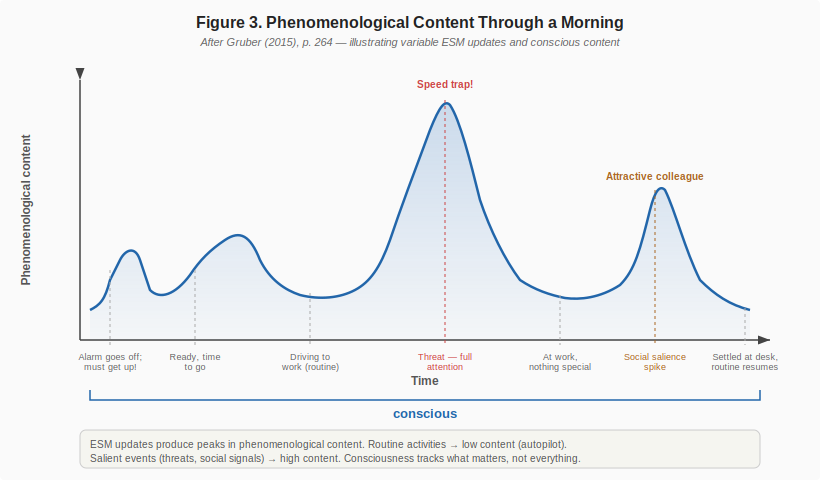
\includegraphics[width=0.85\textwidth]{figure3-phenomenological-content.png}
\caption{The structure of phenomenological content: what appears in the virtual world (EWM) and how the virtual self (ESM) experiences it. The boundary between implicit and explicit determines what reaches conscious awareness.}
\label{fig:phenomenological}
\end{figure}

Two independent paths---theoretical reasoning from computational first principles \citep{Gruber2015} and large-scale empirical neuroscience \citep{HengenShew2025,AlgomShriki2026}---converging on the same claim a decade apart. This convergence does not prove the Four-Model Theory correct, but it provides substantial independent support for one of its core predictions.

The Four-Model Theory distinguishes two thresholds for consciousness:
\begin{itemize}
\item \textbf{Physical threshold}: Criticality. The substrate must operate at Class~4 dynamics. Below this, no consciousness is possible regardless of architecture.
\item \textbf{Functional threshold}: Four-model architecture. The substrate must implement the four-model self-simulation. Above criticality but without the architecture, there is complex dynamics but no consciousness.
\end{itemize}

Both thresholds must be met. Criticality is necessary but not sufficient; the four-model architecture is necessary but not sufficient. Together they are sufficient.

\subsection{The Meta-Problem Dissolved}

The Meta-Problem---why we think there is a Hard Problem---receives a natural account within the Four-Model Theory. The ISM (Implicit Self Model) is \textbf{structurally inaccessible} to the ESM (Explicit Self Model). The conscious self cannot directly observe its own substrate. When the ESM attempts to model the basis of its own experience, it encounters a principled opacity: the implicit models that generate the simulation are not themselves part of the simulation.

This is why consciousness \textit{seems} mysterious. The ESM can represent that it is having an experience, but it cannot represent the mechanism by which the experience is generated---because that mechanism operates at the implicit/substrate level, which is by definition outside the explicit/virtual level. The result is the persistent intuition that something is being ``left out'' of any physical explanation: the ESM cannot find the mechanism within its own simulation, so it concludes the mechanism must be non-physical or fundamentally inexplicable.

This account shares features with Graziano's AST explanation---both invoke the self-model's necessary incompleteness---but grounds it in a more specific architecture (four models, real/virtual split) and connects it to the broader dissolution of the Hard Problem rather than treating the Meta-Problem in isolation.

%=============================================================================
\section{Philosophical Commitments}
%=============================================================================

The Four-Model Theory entails specific philosophical positions that were established through structured adversarial analysis and are internally consistent. This section develops and defends each commitment.

\subsection{Process Physicalism}

The theory is physicalist: both substrate and simulation are physical processes. Qualia are patterns of activity within the simulation constituting the ESM's self-perception. This is process physicalism: consciousness is constituted by the \textit{process} of self-simulation, not identical to any particular neural state. The same conscious state could be realized by different substrates---what matters is the functional architecture (four models at criticality), not the material.

Process physicalism adds the real/virtual level distinction to standard functionalism, which is what allows it to address phenomenality: qualia are not just functional roles but virtual properties of the simulation---genuinely experiential but not properties of the substrate.

\subsection{Epiphenomenalism}

The theory commits to epiphenomenalism: consciousness \textbf{observes but does not cause}. The substrate-level architecture is causally efficacious; the experience that accompanies it does not feed back to influence operations. This entails that \textbf{free will is an illusion}: the ESM narrates decisions already made at the substrate level \citep{Libet1985,Schurger2012,Wegner2002}. However, reflecting on free will can alter the substrate's future decision landscape, creating something functionally close to the libertarian ideal without top-down phenomenal causation.

\textbf{Why does consciousness exist if epiphenomenal?} The \textit{architecture} is selected for, not the \textit{experience}. Natural selection targets the functional capabilities (predictive modeling, social cognition); consciousness is a necessary accompaniment, not a separate target.

This framing addresses the main objections. \textbf{Zombies} \citep{Chalmers1996}: not possible---the virtual models \textit{are} the substrate's activity at the virtual level, just as a vortex is not added to water's movement but is a description of it. \textbf{The knowledge argument} \citep{Jackson1982}: Mary gains acquaintance with a virtual quale she could not access from substrate descriptions---real knowledge, no causal power required. \textbf{The evolutionary argument}: the architecture is selected for; consciousness comes along necessarily.

\subsection{Weak Emergence}

Consciousness is weakly emergent: deducible in principle from a complete substrate description, even if practically irreducible. No strong emergence, no magical threshold. This avoids both strong emergence difficulties \citep{Kim1993} and the panpsychist Combination Problem \citep{Chalmers2016}. Consciousness arises from the computational properties of a system running a self-simulation at criticality, as a weather pattern arises from atmospheric thermodynamics---no extra ingredient needed.

\subsection{Substrate Independence}

The six-layer mammalian neocortex is one evolutionary implementation of the four-model architecture---a highly successful one, but not the only possible one. Consciousness is substrate-independent: any physical system capable of implementing the four-model architecture at criticality should produce consciousness, regardless of its material composition.

Biological evidence already supports this. Corvids (crows, ravens) and parrots demonstrate cognitive abilities---tool use, future planning, mirror self-recognition, social deception---that strongly suggest consciousness, yet their brains have no neocortex. Their pallium is organized in nuclear clusters rather than layers \citep{Gunturkun2016}. Cephalopods (octopuses) demonstrate problem-solving, tool use, and behavioral flexibility with an even more radically different brain architecture---a largely decentralized nervous system with more neurons in the arms than in the central brain. If the Four-Model Theory is correct, these animals are conscious not because they share our neural architecture but because they have evolved functionally equivalent self-simulation architectures on different substrates---exactly what substrate independence predicts.

The implication for artificial consciousness is direct: a synthetic system implementing the four-model architecture at criticality should produce genuine consciousness (see Section~8, Prediction~7 and Section~10.1). Current AI systems, including large language models, do not meet this specification. LLMs lack an Explicit Self Model (they do not run a real-time self-simulation), lack criticality (transformer inference is a feedforward pass---Class~1/2 dynamics), and lack the real/virtual split that grounds phenomenality. The theory predicts that the qualitative difference between interacting with a genuinely conscious artificial system and interacting with an LLM would be immediately and qualitatively distinguishable.

%=============================================================================
\section{Binding, Criticality, and Holographic Storage}
%=============================================================================

\subsection{Binding as an Emergent Property of Critical Dynamics}

Binding is not a separate mechanism but an emergent property of criticality. At the edge of chaos, maximal correlation length means distant substrate regions influence each other and information integrates across the network. Binding is a consequence of the dynamical regime, not an additional computation. This is consistent with gamma-band synchrony \citep{Fries2005,Fries2015}, long-range thalamocortical coherence \citep{Llinas1998}, and criticality signatures \citep{Beggs2003,Tagliazucchi2012}.

\subsection{Holographic Storage}

The implicit models (IWM, ISM) store information in a distributed, non-local manner---standard distributed representations \citep{Hinton1986} where each piece of information is spread across many connection weights and each weight participates in storing many pieces of information. This produces graceful degradation: partial damage reduces quality but does not eliminate specific memories or skills.

The term ``holographic'' is used as analogy: just as cutting a hologram in half produces two complete but lower-resolution images, splitting a distributed network produces two degraded but functionally complete copies. This property is critical for understanding split-brain phenomena (Section~6.4) and makes the specific prediction that callosotomy should produce bilateral but degraded function, not clean lateralized loss.

\subsection{Consciousness States Derived from Criticality}

The criticality requirement provides a unified account of when consciousness is present and when it is absent. Consciousness tracks the substrate's position relative to the critical point:

\begin{table}[htbp]
\centering
\caption{Consciousness States and Criticality}
\label{tab:consciousness-states}
\small
\renewcommand{\arraystretch}{1.4}
\begin{tabularx}{\textwidth}{>{\raggedright}p{1.9cm} >{\raggedright}p{1.7cm} >{\raggedright}p{3.2cm} X >{\raggedright\arraybackslash}p{2cm}}
\toprule
\textbf{State} & \textbf{Criticality} & \textbf{Four-model status} & \textbf{Consciousness prediction} & \textbf{Key evidence} \\
\midrule
Normal waking & At/near critical & All four active & Full consciousness & High PCI \\
REM sleep & Near-critical & EWM/ESM on internal input & Degraded (dream) & Moderate PCI \\
Deep NREM & Subcritical & EWM/ESM collapse & Absent & Low PCI \\
Propofol & Forced subcritical & EWM/ESM suppressed & Absent & PCI $\approx$ 0 \\
Ketamine & NOT subcritical & EWM/ESM on wrong input & Present but disconnected & Increased entropy \\
Psychedelics & At/past critical & All active, permeability $\uparrow$ & Present, altered & Enhanced complexity \\
Vegetative state & Typically subcritical & EWM/ESM collapsed & Absent (usually) & Low metabolism \\
Covert awareness & At criticality & EWM/ESM intact, output damaged & Present but unexpressible & Owen et al.\ \\
MCS & Fluctuating & Intermittent EWM/ESM & Intermittent & Fluctuating PCI \\
\bottomrule
\end{tabularx}
\end{table}

The key distinction is between \textbf{propofol} and \textbf{ketamine}. Propofol pushes the substrate subcritical $\to$ no consciousness \citep{Alkire2000,Boly2012}. Ketamine does \textit{not} push subcritical---it increases neural entropy \citep{Schartner2015}---but disrupts sensory processing, so the EWM and ESM operate on distorted signals: consciousness present but disconnected \citep{Corlett2013}. What matters is not pharmacological classification but the effect on the substrate's dynamical regime.

%=============================================================================
\section{Explanatory Range}
%=============================================================================

A theory's value lies partly in its ability to derive diverse phenomena from a small set of principles. The Four-Model Theory's five principles---criticality, virtual qualia, redirectable ESM, variable implicit--explicit permeability, and virtual model forking---generate accounts of phenomena across psychopharmacology, clinical neurology, sleep science, comparative cognition, and clinical psychology. This section demonstrates that range.

\subsection{Psychedelic Phenomenology}

Psychedelics produce a characteristic profile: visual intensification, synesthesia, enhanced pattern recognition, ego dissolution at high doses, and radical identity alteration \citep{CarhartHarris2012,CarhartHarris2016,Timmermann2019,Timmermann2023}. The theory accounts for this through three mechanisms.

\textbf{Implicit--explicit permeability increase}. Psychedelics increase the global permeability of the implicit--explicit boundary. Intermediate processing stages---normally implicit and inaccessible---leak through to the simulation, producing an ordered visual progression: V1-level (phosphenes, enhanced contrast) $\to$ V2/V3-level (geometric patterns, form constants; \citealp{Kluver1966}) $\to$ higher visual areas (faces, figures, scenes) $\to$ complex dream-like visions. This progression follows the visual processing hierarchy in a predictable, dose-dependent order---a direct consequence of the permeability gradient propagating up the hierarchy.

\textbf{Ego dissolution = ESM redirection, not abolition}. At high doses, the ESM loses its normal self-referential input but continues to run, latching onto whatever dominates the available input stream. This produces ego dissolution: the feeling that the boundary between self and world has dissolved. Critically, this predicts that ego dissolution \textit{content} is not random but determined by the dominant input. This is dramatically confirmed by \textbf{salvia divinorum} phenomenology: users reliably report ``becoming'' objects in their environment---furniture, walls, characters from television playing in the room. The ESM, deprived of self-input, latches onto whatever sensory input dominates. The identity experience tracks input in a predictable, controllable manner---no competing theory generates this prediction (Section~8, Prediction~3).

\textbf{Intensity as novelty}. Psychedelic profundity reflects increased \textit{novel content}, not increased consciousness level---the permeability increase floods the simulation with normally implicit information.

\subsection{Anesthesia and Clinical Disorders}

\textbf{Propofol anesthesia}: Pushes the substrate subcritical $\to$ consciousness abolished (Table~3). \textbf{Ketamine}: Does not push subcritical---it increases neural entropy \citep{Schartner2015}---but disrupts sensory processing, so the EWM and ESM operate on distorted signals: consciousness present but disconnected \citep{Corlett2013}. The key distinction: what matters is not pharmacological classification but the effect on the substrate's dynamical regime.

\textbf{Vegetative state vs.\ covert awareness}: If the substrate is subcritical $\to$ no consciousness. But if the substrate is at criticality with damaged \textit{output pathways}, consciousness is present but unexpressible---precisely \textbf{cognitive motor dissociation} (CMD), documented by \citet{Owen2006} and \citet{Monti2010}, in which patients clinically diagnosed as vegetative demonstrate awareness through brain-imaging paradigms. The theory predicts that the distinction between truly vegetative (subcritical substrate) and covertly conscious (critical substrate with damaged output) should be detectable via criticality measures such as PCI \citep{Casali2013,Casarotto2016}. \textbf{Minimally conscious state}: the substrate fluctuates around the criticality threshold $\to$ intermittent consciousness, explaining characteristic behavioral variability.

\textbf{Cotard's delusion}: Patients report believing they are dead or that their organs have disappeared. The ESM receives severely distorted interoceptive input (due to neurological damage or psychiatric disorder) and constructs ``I am dead'' as its best model of the absence of normal embodied signals---the same redirectable-ESM mechanism that produces ``I am a chair'' under salvia, applied to a clinical context.

\textbf{Anosognosia}: Patients with anosognosia (typically following right-hemisphere stroke) are unaware of their own deficits---they deny being paralyzed or impaired, even in the face of clear evidence. The theory explains this as a \textbf{local decrease in implicit--explicit permeability}: the ISM contains the deficit information but transfer to the EWM is blocked for that specific domain. The patient's simulation simply does not include the deficit, so the patient genuinely does not experience it. This is the \textbf{inverse} of the psychedelic mechanism: psychedelics globally increase permeability, while anosognosia locally decreases it. The theory connects these phenomena under a single principle---variable permeability---and predicts psychedelics should alleviate anosognosia by compensating for the local block with a global permeability increase (Section~8, Prediction~4).

\textbf{Dissociative Identity Disorder (DID)}: The virtual models, being software-like, can be \textbf{forked}. DID represents a substrate running multiple ESM configurations---multiple self-models---that alternate in controlling the simulation. Each alter is a distinct configuration of the ESM, with its own self-narrative, emotional profile, and behavioral patterns, running on the same substrate. The theory predicts that distinct alters should correspond to distinct patterns of neural activity, detectable with neuroimaging (Section~8, Prediction~9).

\subsection{Dreams}

Dreaming represents the simulation running in \textbf{degraded mode}: near-critical dynamics (sufficient for consciousness) but with external input cut off (sensory deprivation during sleep).

The EWM continues to generate a world---but without the constraint of sensory input, the simulation draws on the IWM's stored knowledge, producing the characteristic features of dreams: familiar places and people, impossible physics, narrative incoherence, and emotional intensity. The ESM continues to generate a self---you experience dreams as happening to ``you''---but with reduced metacognitive oversight, producing the characteristic lack of insight in dreams (you accept impossible events without question).

\textbf{Lucid dreaming} provides direct evidence for the software-like quality of the virtual models. In a lucid dream, the dreamer becomes aware that they are dreaming: the ESM ``toggles on'' more fully, gaining metacognitive access within the dream state. The theory predicts lucid dream onset corresponds to a \textbf{criticality threshold crossing}---a step-like increase in neural complexity as the ESM activates more fully, detectable as a discontinuity in EEG complexity measures (Section~8, Prediction~8).

The criticality framework also explains the \textbf{NREM/REM transition}: as the brain's dynamical state fluctuates during sleep, crossing the criticality threshold produces the transition from non-conscious deep sleep to conscious dreaming. The 90-minute ultradian cycle corresponds to an oscillation of the substrate around the critical point.

\subsection{Split-Brain}

Callosotomy produces the classic split-brain syndrome \citep{Gazzaniga1962,Gazzaniga2000}. Because the implicit models store information holographically (Section~5.2), physical separation does not cleanly divide the models into left and right halves. Instead, it produces \textbf{two degraded but functionally complete copies}. Each hemisphere retains a degraded version of the IWM, ISM, EWM, and ESM---complete enough to sustain consciousness but lacking the resolution and scope of the intact system.

This accounts for the key features of split-brain behavior:
\begin{itemize}
\item \textbf{Each hemisphere sustains independent consciousness}: Both are above the criticality threshold and both have complete (if degraded) four-model architectures.
\item \textbf{The left hemisphere interpreter} \citep{Gazzaniga2000}: The left hemisphere's ESM confabulates explanations for behavior initiated by the right hemisphere. This is the \textit{same confabulation mechanism} observed in Cotard's delusion, anosognosia, and salvia experiences: an ESM constructing the best narrative it can from incomplete input.
\item \textbf{Degradation rather than clean division}: Split-brain patients do not show perfectly hemispheric specialization; they show graded deficits \citep{Pinto2017}, consistent with holographic degradation rather than binary splitting.
\end{itemize}

\subsection{Animal Consciousness}

The theory's commitments---continuum (not binary), substrate independence, criticality threshold---predict a \textbf{gradient} of animal consciousness. Mammals implement the four-model architecture in graduated form, with even simple cortices (rodents) supporting basic consciousness---rudimentary simulation sufficient for phenomenal experience but thin in self-awareness.

\textbf{Corvids and parrots} present a crucial test case: tool manufacture, mirror self-recognition, social deception, and future planning---yet no neocortex, with pallium organized in nuclear clusters \citep{Gunturkun2016}. The theory predicts these animals are conscious because they have evolved functionally equivalent self-simulation architectures on a different substrate. \textbf{Cephalopods} extend this logic further, with largely decentralized nervous systems that should produce consciousness with unusual features. Both cases test substrate independence directly.

\subsection{Clinical Psychology Bridge}

\textbf{CBT} works as virtual model reprogramming: repeated corrective experience drives substrate-level rewiring (synaptic plasticity), modifying the ISM, which changes the ESM's self-model. \textbf{Phobias} are EWM misconfigurations where threat representation exceeds the IWM's evidence base; exposure therapy updates the IWM to correct the EWM.

\textbf{The placebo effect} is consistent with epiphenomenalism: placebo activates substrate-level expectation circuits (endogenous opioid release) that operate in parallel with---not caused by---the conscious experience of hope. The correlation between conscious expectation and physical effect is real but non-causal: both are products of the same substrate processes.

\textbf{Conversion disorder} is the inverse of blindsight: in blindsight, the substrate processes visual information without including it in the EWM; in conversion disorder, the EWM models a deficit (paralysis, blindness) that the intact substrate does not have.

%=============================================================================
\section{Comparative Analysis}
%=============================================================================

This section provides a systematic comparison between the Four-Model Theory and six major competitors across the eight requirements established in Section~2. The comparison aims to be fair: each theory's genuine strengths are acknowledged, and the Four-Model Theory's advantages are located precisely.

\subsection{Scoring Matrix}

Table~4 presents an assessment of how each theory addresses the eight requirements. All ratings reflect the present author's judgment. Ratings: $\bullet$ = addresses, \textcircled{\raisebox{-0.3pt}{\footnotesize\textbf{--}}} = partial, $\circ$ = minimal, --- = silent, n/a = not applicable.

\begin{table}[htbp]
\centering
\caption{Theory Comparison Across Eight Requirements}
\label{tab:comparison}
\small
\begin{tabular}{lccccccc}
\toprule
\textbf{Requirement} & \textbf{FMT} & \textbf{IIT} & \textbf{GNW} & \textbf{HOT} & \textbf{PP} & \textbf{AST} & \textbf{RPT} \\
\midrule
Hard Problem & $\bullet$ & $\bullet^\dagger$ & ---$^\ddagger$ & \textcircled{\raisebox{-0.3pt}{\footnotesize\textbf{--}}} & ---$^\ddagger$ & \textcircled{\raisebox{-0.3pt}{\footnotesize\textbf{--}}} & --- \\
Expl.\ Gap & $\bullet$ & $\bullet^\dagger$ & ---$^\ddagger$ & \textcircled{\raisebox{-0.3pt}{\footnotesize\textbf{--}}} & ---$^\ddagger$ & \textcircled{\raisebox{-0.3pt}{\footnotesize\textbf{--}}} & --- \\
Boundary & $\bullet$ & $\bullet$ & \textcircled{\raisebox{-0.3pt}{\footnotesize\textbf{--}}} & $\circ$ & \textcircled{\raisebox{-0.3pt}{\footnotesize\textbf{--}}} & \textcircled{\raisebox{-0.3pt}{\footnotesize\textbf{--}}} & \textcircled{\raisebox{-0.3pt}{\footnotesize\textbf{--}}} \\
Structure & $\bullet$ & $\bullet$ & \textcircled{\raisebox{-0.3pt}{\footnotesize\textbf{--}}} & \textcircled{\raisebox{-0.3pt}{\footnotesize\textbf{--}}} & $\bullet$ & \textcircled{\raisebox{-0.3pt}{\footnotesize\textbf{--}}} & \textcircled{\raisebox{-0.3pt}{\footnotesize\textbf{--}}} \\
Binding & $\bullet$ & $\bullet$ & \textcircled{\raisebox{-0.3pt}{\footnotesize\textbf{--}}} & $\circ$ & \textcircled{\raisebox{-0.3pt}{\footnotesize\textbf{--}}} & $\circ$ & \textcircled{\raisebox{-0.3pt}{\footnotesize\textbf{--}}} \\
Combination & $\bullet$ & $\circ^{\dagger\dagger}$ & n/a & n/a & n/a & n/a & n/a \\
Causal Role & $\bullet$ & \textcircled{\raisebox{-0.3pt}{\footnotesize\textbf{--}}} & \textcircled{\raisebox{-0.3pt}{\footnotesize\textbf{--}}} & \textcircled{\raisebox{-0.3pt}{\footnotesize\textbf{--}}} & $\bullet$ & \textcircled{\raisebox{-0.3pt}{\footnotesize\textbf{--}}} & $\bullet$ \\
Meta-Problem & $\bullet$ & $\circ$ & \textcircled{\raisebox{-0.3pt}{\footnotesize\textbf{--}}} & \textcircled{\raisebox{-0.3pt}{\footnotesize\textbf{--}}} & \textcircled{\raisebox{-0.3pt}{\footnotesize\textbf{--}}} & $\bullet$ & $\circ$ \\
\bottomrule
\end{tabular}

\smallskip
\noindent\footnotesize
$^\dagger$\,Axiomatic identification; debated whether this is a solution or redefinition. \enspace
$^{\dagger\dagger}$\,Panpsychist commitments lead to the Combination Problem \citep{Chalmers2016}. \enspace
$^\ddagger$\,GNW and PP proponents argue these theories address the ``real problem'' of consciousness \citep{Seth2021}; the ``silent'' rating reflects the scope of the requirement as defined in \S2.
\end{table}

\subsection{Theory-by-Theory Comparison}

\textbf{IIT} \citep{Tononi2004,Albantakis2023}: Strengths in mathematical rigor, qualia space, and principled boundary-setting (exclusion postulate). However, its axiom-based identification of consciousness with $\Phi$ leads to panpsychist consequences, the Combination Problem remains unresolved \citep{Chalmers2016}, $\Phi$ is computationally intractable \citep{Aaronson2014}, and the unfolding argument \citep{Doerig2019} challenges its central claim. The Four-Model Theory avoids panpsychism, has no combination problem (weak emergence), and generates predictions without computing $\Phi$.

\textbf{GNW} \citep{Baars1988,Dehaene2011}: Clear, empirically tractable account of access consciousness. But silent on the Hard Problem---explaining \textit{when} but not \textit{why} broadcast produces experience. The COGITATE results (2025) were problematic: posterior cortex showed stronger consciousness-related activity than the frontoparietal workspace. The Four-Model Theory agrees that broadcasting is mechanistically important but adds the real/virtual distinction that addresses phenomenality.

\textbf{HOT} \citep{Rosenthal2005,Lau2011}: Naturally explains which states are conscious (those with higher-order representations). But does not address binding, leaves the Hard Problem partially treated (why does higher-order representation produce phenomenality?). The Four-Model Theory shares HOT's emphasis on self-representation but embeds it in the richer four-model architecture, explaining \textit{why} self-representation produces phenomenality.

\textbf{PP} \citep{Seth2021}: Strong on experiential structure and causal role (via active inference). Seth's controlled hallucination framework is among the most empirically productive in the field. But explicitly silent on the Hard Problem (Seth, 2021, acknowledges this). The Four-Model Theory adds the architecture, criticality requirement, and real/virtual distinction that PP lacks.

\textbf{AST} \citep{Graziano2013}: Strongest Meta-Problem account but deflationary about phenomenality and does not address binding. The Four-Model Theory incorporates AST's insight while adding the virtual qualia framework that explains \textit{why} phenomenality exists, not just why we think it does.

\textbf{RPT} \citep{Lamme2006}: Empirically specific with strong support from visual masking paradigms. But silent on the Hard Problem and limited to visual consciousness. Compatible at the mechanistic level---recurrent processing likely implements the real-time simulation.

\subsection{Emerging Frameworks (2024--2026)}

\textbf{Biological computationalism} \citep{Milinkovic2025} challenges substrate independence. The Four-Model Theory treats this as empirical: corvids with non-cortical brain architecture \citep{Gunturkun2016} already favor substrate independence. The \textbf{Multiple Generator Hypothesis} \citep{KirkebyHinrup2025} is potentially compatible: the four models could be understood as distinct generators unified by criticality.

\subsection{Summary of Comparative Advantages}

The theory's advantages are: (1) dissolving the Hard Problem without panpsychism or strong emergence; (2) unifying binding with criticality; (3) the redirectable ESM for identity-content prediction; (4) connecting psychedelics and anosognosia under variable permeability; (5) the Meta-Problem as structural consequence. Its primary disadvantage is the absence of mathematical formalization (see Section~9).

%=============================================================================
\section{Novel Testable Predictions}
%=============================================================================

A theory is only as valuable as the predictions it generates. The Four-Model Theory yields nine novel testable predictions, several of which are unique---no competing theory can generate them.

\subsection{Prediction 1: Distinct fMRI Signatures for Each Model}

\textbf{Statement}: If the four models are functionally distinct processes, tasks that selectively engage a single model should produce distinct, reproducible neural activation patterns detectable via fMRI. IWM-dominant tasks (implicit priming, passive recognition) should activate different networks than ISM-dominant tasks (habitual motor sequences, implicit body-schema tasks), which should differ from EWM-dominant tasks (active perceptual discrimination, novel scene processing) and ESM-dominant tasks (self-reflection, agency judgments, mirror self-recognition).

\textbf{Mechanism}: The implicit models (IWM, ISM) should preferentially engage substrate-level storage networks (hippocampal-cortical for IWM, somatosensory-cerebellar for ISM), while the explicit models (EWM, ESM) should preferentially engage simulation networks (sensory cortices for EWM, default mode network and medial prefrontal cortex for ESM).

\textbf{Testability}: High. Design a factorial task battery crossing scope (world vs.\ self) with mode (implicit vs.\ explicit), yielding four conditions. Contrast activation maps across conditions using standard fMRI subtraction or multivariate pattern analysis. The prediction is a double dissociation: scope $\times$ mode interaction effects in distributed networks. \textbf{Unique}: Yes---the specific 2$\times$2 factorial structure is mandated only by this theory.

\subsection{Prediction 2: Psychedelic Content Maps the Processing Hierarchy}

Under psychedelics, visual content progresses through the cortical hierarchy in a dose-dependent sequence: V1 (phosphenes) $\to$ V2/V3 (form constants) $\to$ higher areas (faces, figures) $\to$ complex scenes. \textbf{Testability}: High (graded dosing + concurrent fMRI/MEG). Partial evidence exists \citep{CarhartHarris2016,Timmermann2023} but has not been systematically tested as dose-correlated progression. \textbf{Unique}: Partially---PP predicts hierarchical effects but not the specific ordered sequence.

\subsection{Prediction 3: Ego Dissolution Content Is Controllable}

\textbf{Statement}: During psychedelic ego dissolution, the content of the altered identity experience (what the subject ``becomes'') tracks the dominant sensory input. By controlling the sensory environment during ego dissolution, the identity content can be predicted and directed.

\textbf{Mechanism}: The ESM, deprived of normal self-referential input, latches onto whatever input dominates the available stream. Control the input $\to$ control the identity content.

\textbf{Testability}: High. Administer ego-dissolution-inducing doses of psilocybin or salvia divinorum under controlled conditions. Vary the dominant sensory input (specific visual scenes, specific auditory environments, specific tactile inputs) across conditions. Measure correspondence between controlled input and reported identity content.

\textbf{Unique}: \textbf{Yes---no competing theory can generate this prediction.} IIT, GNW, HOT, PP, and AST have no mechanism for specifying what a subject will ``become'' during ego dissolution. This is the theory's most distinctive empirical prediction.

\subsection{Prediction 4: Psychedelics Alleviate Anosognosia}

\textbf{Statement}: Administration of psychedelic substances at sub-ego-dissolution doses should alleviate anosognosia by globally increasing implicit--explicit permeability, compensating for the local permeability block that causes deficit unawareness.

\textbf{Mechanism}: Anosognosia = local permeability block. Psychedelics = global permeability increase. The global increase should overwhelm the local block, allowing the deficit information in the ISM to reach the EWM.

\textbf{Testability}: Medium (requires clinical trial with stroke patients). Could begin with case studies or observational reports of psychedelic use by patients with anosognosia. Psilocybin-assisted therapy is already being tested for various neuropsychiatric conditions, providing a potential clinical pathway.

\textbf{Unique}: \textbf{Yes---this is a cross-domain surprise prediction.} No other theory connects psychedelics and anosognosia through a single mechanism. Confirmation would be strong evidence for the variable-permeability principle.

\subsection{Prediction 5: All Anesthetics Converge on Criticality Disruption}

\textbf{Statement}: Despite diverse receptor-level mechanisms (GABAergic, NMDA, opioid, $\alpha_2$-adrenergic), all agents that abolish consciousness do so by pushing the substrate below the criticality threshold. Agents that alter but do not abolish consciousness (ketamine, low-dose psychedelics) do not push below criticality.

\textbf{Mechanism}: The criticality requirement is the physical threshold for consciousness; any mechanism that disrupts criticality disrupts consciousness, regardless of receptor pathway.

\textbf{Testability}: High. Measure criticality indicators (PCI, Lempel-Ziv complexity, power-law exponents, detrended fluctuation analysis) across the full range of anesthetic agents at equi-potent doses. The prediction is that abolition of consciousness always correlates with subcriticality, and preserved consciousness (even if altered) always correlates with maintained criticality.

\textbf{Unique}: Shared with the ConCrit framework \citep{AlgomShriki2026}. However, the Four-Model Theory predicted this from theoretical first principles \citep{Gruber2015}, prior to the empirical consolidation.

\subsection{Prediction 6: Split-Brain Produces Holographic Degradation}

\textbf{Statement}: After callosotomy, each hemisphere retains a degraded but functionally \textit{complete} set of cognitive and experiential capacities---not a clean hemispheric specialization. The degradation should be proportional to the extent of commissural severing (partial callosotomy $\to$ partial degradation).

\textbf{Mechanism}: Holographic storage. Information is distributed across the full substrate; cutting connections degrades both copies but does not destroy either.

\textbf{Testability}: High. Systematic cognitive assessment of split-brain patients across domains, testing for the predicted pattern of bilateral but degraded capabilities rather than clean lateralization. \citet{Pinto2017} provide preliminary evidence. \textbf{Unique}: Yes---the Four-Model Theory provides the theoretical basis (holographic storage) and predicts the specific pattern (graded degradation proportional to disconnection, not binary split).

\subsection{Prediction 7: Artificial Consciousness via Four Models at Criticality}

\textbf{Statement}: A synthetic system implementing the four-model architecture at criticality will exhibit consciousness. The qualitative difference between interacting with such a system and interacting with a current LLM will be immediately and qualitatively distinguishable.

\textbf{Mechanism}: Substrate independence. Consciousness depends on function (four models at criticality), not on material (biological neurons). Current LLMs fail on multiple counts: feedforward inference (Class~1/2 dynamics, far below criticality), no ISM/ESM (no real-time self-simulation constituting a subjective perspective), and no real/virtual split.

\textbf{Testability}: Medium (requires significant engineering development). However, intermediate tests are possible: systems with partial implementations (e.g., two models instead of four, or four models without criticality) should show partial consciousness indicators, detectable through behavioral signatures and computational complexity measures.

\textbf{Unique}: Yes---provides a specific architectural blueprint, unlike PP or GNW which are compatible with artificial consciousness but do not specify a design.

\subsection{Prediction 8: Lucid Dream Onset Is a Criticality Threshold Crossing}

\textbf{Statement}: The transition from non-lucid to lucid dreaming corresponds to a step-like increase in neural complexity, consistent with the substrate crossing a criticality threshold. This should be detectable as a discontinuity in EEG complexity measures, not a gradual change.

\textbf{Mechanism}: Lucid dreaming = ESM activation within the dream state. ESM activation requires sufficient criticality to support the additional level of self-modeling.

\textbf{Testability}: High. EEG/polysomnographic recording with concurrent signaling by lucid dreamers (established paradigm; \citealp{LaBerge1985}). Analyze complexity measures (PCI, Lempel-Ziv, spectral exponents) in a time-locked window around signaled onset of lucidity. \textbf{Unique}: Partially---the specific prediction of a step-like discontinuity (reflecting threshold-crossing rather than gradual increase) is distinctive.

\subsection{Prediction 9: DID Alters Have Distinct Neural Signatures}

\textbf{Statement}: Different alters in DID correspond to distinct, measurable configurations of neural activity---not merely behavioral differences or different self-reports, but different neural dynamics detectable through neuroimaging.

\textbf{Mechanism}: Virtual model forking. Each alter is a distinct configuration of the ESM, running on the same substrate but with different parameters. Different parameters should produce different activity patterns.

\textbf{Testability}: High. fMRI or EEG recording during controlled alter switching in DID patients. Compare within-patient across-alter variability against within-patient within-alter variability. The prediction is that across-alter variability will be significantly greater and will show consistent alter-specific patterns. Differences should localize to ESM-related networks (default mode, medial prefrontal, posterior cingulate). \textbf{Unique}: Yes---the Four-Model Theory provides the theoretical basis (ESM forking) for predicting \textit{consistent, alter-specific neural signatures} rather than merely \textit{differences} (cf.\ \citealp{Reinders2006,Reinders2014}).

\subsection{The Ultimate Prediction}

If the Four-Model Theory is correct, it should be possible to \textit{build} a conscious machine by implementing the specified architecture: four nested models (IWM, ISM, EWM, ESM) operating at criticality on a substrate of sufficient complexity. The theory predicts that such a system would not merely simulate consciousness but would \textit{be} conscious---would have genuine phenomenal experience constituted by its virtual models.

This prediction is not currently testable---the engineering does not yet exist, and even if it did, the other-minds problem would make verification philosophically difficult. However, the prediction sets a bold bar: if the theory is correct, the difference between interacting with a conscious artificial system and interacting with any current AI should be qualitatively obvious to human observers---a difference in \textit{kind}, not merely in degree.

%=============================================================================
\section{Open Questions}
%=============================================================================

Intellectual honesty requires identifying what the theory does not yet resolve. These are research frontiers, not theoretical weaknesses---they are questions that arise \textit{from} the theory and that the theory's framework helps to sharpen.

\textbf{1.\ Are all four models virtual?} The theory describes the implicit models (IWM, ISM) as ``real side'' and the explicit models (EWM, ESM) as ``virtual side.'' But it is not certain that this division is sharp. The implicit models might themselves have virtual properties---they are, after all, \textit{models}, not raw physics. If the implicit models are also virtual in some sense, what constitutes the ``real side''? This is an open question even for the theory's author, and its resolution may have consequences for the Hard Problem treatment.

\textbf{2.\ Mathematical formalization.} The criticality requirement is specified qualitatively (Wolfram's Class~4 regime), not quantitatively. A full mathematical treatment---defining the four models formally, specifying the criticality threshold in terms of measurable quantities, deriving the predictions as formal consequences---remains to be developed. ConCrit's mathematical tools (power-law exponents, detrended fluctuation analysis, branching parameters) provide a starting point, as do the formal tools of dynamical systems theory and information geometry.

\textbf{3.\ Physical implementation.} Which physical mechanism in the biological brain supports criticality? Candidates include cortical column dynamics, thalamocortical standing waves, glial modulation, and (more speculatively) quantum processes in microtubules \citep{PenroseHameroff1994}, though see \citet{Tegmark2000} for decoherence objections. The theory is agnostic: it specifies the \textit{functional} requirements without mandating a specific physical mechanism.

\textbf{4.\ Minimum configuration.} Can the four models partially dissociate? Is it possible to have an EWM without an ESM (world-experience without self-experience), or an ESM without an EWM? What is the minimum set of models required for consciousness? The graduated levels (Section~3.5) suggest a hierarchy, but the exact minimum configuration may require simulation or empirical investigation to determine.

%=============================================================================
\section{Discussion}
%=============================================================================

\subsection{Implications for Artificial Consciousness}

The Four-Model Theory provides an engineering specification for artificial consciousness: implement the four-model architecture on a substrate operating at criticality. This is a concrete deliverable, not an abstract philosophical claim.

Current AI systems fail this specification in at least two ways. Large language models (LLMs) operate via feedforward inference (transformer attention is computed in a single pass without recurrent dynamics), which corresponds to Wolfram's Class~1/2---far below the criticality threshold. They also lack the four-model architecture: there is no ISM (no substrate-level self-knowledge that is \textit{distinct from} the model's outputs), no ESM (no real-time self-simulation that constitutes a subjective perspective), and no real/virtual split (no two-level ontology in which experience resides at the virtual level).

This does not mean that LLMs are necessarily non-conscious---the theory cannot prove a negative---but it predicts that they lack the architecture required for consciousness as the theory defines it. The growing discourse around AI consciousness \citep{Butlin2023,Butlin2025,Schwitzgebel2025,Birch2025} and AI welfare \citep{Long2024,Anthropic2025} makes this distinction practically important. A theory that provides clear criteria for artificial consciousness---rather than vague analogies to human cognition---has immediate ethical and engineering value.

\subsection{Implications for Consciousness Science}

The Four-Model Theory suggests a shift in experimental priorities. Rather than adjudicating between IIT and GNW (the current focus of adversarial collaborations), the field should:

\begin{enumerate}
\item \textbf{Test the criticality prediction across all anesthetic agents} (Prediction~5)---this is achievable with current methods and would provide strong evidence for or against the criticality framework.
\item \textbf{Design controlled ego-dissolution experiments} (Prediction~3)---the most distinctive prediction, uniquely generated by the redirectable ESM mechanism.
\item \textbf{Investigate the psychedelic--anosognosia connection} (Prediction~4)---a cross-domain prediction that, if confirmed, would constitute strong evidence for the variable-permeability mechanism.
\item \textbf{Measure criticality at lucid dream onset} (Prediction~8)---achievable with established paradigms and equipment.
\end{enumerate}

These experiments do not require committing to the Four-Model Theory in its entirety. They test specific mechanisms (criticality, redirectable ESM, variable permeability) that could be incorporated into other frameworks if confirmed.

\subsection{Limitations}

\textbf{No institutional laboratory.} The predictions presented here were derived theoretically and have not been tested in the author's own laboratory. While this does not affect their validity as predictions, it does mean that empirical testing depends on the willingness of established laboratories to take them up.

\textbf{Epiphenomenalism remains controversial.} The theory's commitment to epiphenomenalism will face resistance from philosophers and scientists who consider it either absurd (consciousness \textit{must} be causally efficacious) or empirically refuted. The defense offered in Section~4.2 is, I believe, sound, but the reader should be aware that this is the theory's most philosophically controversial commitment.

\textbf{Qualitative rather than quantitative.} The theory's predictions are currently stated in qualitative terms (``criticality increases,'' ``permeability changes,'' ``ESM redirects''). Quantitative formalization would strengthen the predictions and enable more precise experimental testing. This is acknowledged as a priority for future work.

\textbf{The other-minds problem.} The ultimate prediction---that a system built to the theory's specification would be conscious---faces the standard other-minds problem: how would we verify consciousness from the outside? Developing consciousness indicators that can be applied to artificial systems is a challenge for the entire field, not specific to this theory.

%=============================================================================
\section{Conclusion}
%=============================================================================

The Four-Model Theory of Consciousness proposes that consciousness is a real-time self-simulation across four nested models---Implicit World Model, Implicit Self Model, Explicit World Model, and Explicit Self Model---operating on a substrate at the edge of chaos. Qualia are virtual: they are the phenomenal properties of the simulation, not of the substrate. This dissolves the Hard Problem by revealing a category error in its formulation, simultaneously closing the Explanatory Gap and accounting for the Meta-Problem.

The theory addresses all eight requirements for a complete theory of consciousness: the Hard Problem (dissolved via virtual qualia), the Explanatory Gap (dissolved alongside), the Boundary Problem (defined by the scope of virtual models), the Structure of Experience (generated by the simulation's complexity), Unity and Binding (emergent from critical dynamics), Combination and Emergence (weak emergence, no combination problem), the Causal Role (architecture is causally efficacious, experience is epiphenomenal), and the Meta-Problem (structural inaccessibility of the ISM to the ESM).

The theory generates nine novel testable predictions, including that ego dissolution content is controllable via sensory input (Prediction~3), that psychedelics should alleviate anosognosia (Prediction~4), and that all consciousness-abolishing anesthetics converge on criticality disruption (Prediction~5). Several of these predictions are unique to the Four-Model Theory---no competing theory can generate them.

The theory's criticality requirement was derived independently from Wolfram's computational framework in 2015, a decade before the empirical literature consolidated the same conclusion---through \citeauthor{HengenShew2025}'s (\citeyear{HengenShew2025}) meta-analysis of 140 datasets and \citeauthor{AlgomShriki2026}'s (\citeyear{AlgomShriki2026}) ConCrit framework. This convergence---theoretical prediction from first principles confirmed by large-scale empirical synthesis---provides strong independent support.

Open questions remain: the status of the implicit models (real or also virtual?), the need for mathematical formalization, the specific physical mechanism supporting criticality, and the minimum configuration for consciousness. These are research frontiers that the theory's framework helps to sharpen.

The ambition of consciousness science is not merely to correlate neural activity with subjective reports but to understand \textit{why} there is experience at all. The Four-Model Theory offers an answer: there is experience because there is a simulation, and within the simulation, experience is not an addition to the process but is constitutive of it. The way to test this answer is not through philosophical argument alone but through the predictions it generates---and ultimately, through the engineering challenge of building a system to the specification and observing whether the result is, as the theory predicts, qualitatively unlike anything that exists today.

%=============================================================================
\section*{Acknowledgments}
%=============================================================================

The theory's adversarial challenge and refinement process was conducted in collaboration with Claude (Anthropic, 2026). Claude served as adversarial interlocutor across ten structured challenge sessions covering the simulation subject problem, ontological status, passive experience, binding, dreams, psychedelics, anesthesia and clinical disorders, split-brain, predictions, and animal consciousness. The theory's scoring on the eight requirements reflects the outcome of this adversarial process. The theory itself is the author's, originally published in 2015; the refinement, stress-testing, and prediction-generation are products of the collaboration.

%=============================================================================
% References
%=============================================================================
\bibliographystyle{plainnat}
\bibliography{references}

\end{document}
